
\documentclass[final,  3p]{elsarticle}


\usepackage{amssymb, amsthm}
\usepackage{amsmath}
\usepackage{subcaption}
\usepackage[T1]{fontenc}
\usepackage{babel}
\usepackage{wrapfig}
\usepackage{geometry}
\usepackage{fancyref}
\usepackage{lineno}
\usepackage{color}
\usepackage{nomencl}
\makenomenclature
\renewcommand{\nomlabel}[1]{\hfil #1\hfil}

\journal{Journal of Quantitative Spectroscopy \& Radiative Transfer}

\begin{document}

\begin{frontmatter}

\title{Investigation of Limited Detection Schemes for Light Scattering of Optically Trapped Asymmetric Particles}


\author[aff1]{Dan Maciver\corref{cor1}} 
\ead{Daniel.Maciver.2016@uni.strath.ac.uk}

\author[aff1]{Praveen Parthasarathi}

\author[aff1]{Leo Lue}

\author[aff1]{Jan Sefcik}

\author[aff1]{Mark Haw}




\cortext[cor1]{Corresponding author}
\affiliation[aff1]{organization={Department of Chemical Engineering,
			University of Strathclyde},
            addressline={75 Montrose Street}, 
            city={Glasgow},
            postcode={G1 1XL}, 
            country={Scotland}}


\begin{abstract}
  % \justifying
  %
  While optical trapping is a well understood method for force
  transduction and detection, further characterisation of trapped entities using light-scattering
  poses a two-fold challenge --- one experimental, concerning the optimal
  arrangement of light detectors to gather data, and the other theoretical, involving
  solving of the inverse light scattering problem in order to interpret this data. Experimentally, combining static
  light scattering techniques with optical trapping poses significant
  engineering challenges due to the space constraints in a
  conventional optical trapping setup.  We propose here a plausible
  scenario of detecting scattered light from an optically trapped
  asymmetric microstructure using a novel, multi-angle, optical-fibre
  based detection scheme and demonstrate how a Bayesian inference
  based analysis of the data, combined with a neural-network trained on data simulated to mimic light scattering
  detection signals in such scenarios, may be used for solving the
  inverse light scattering problem and characterising complex trapped
  entities.  To demonstrate the method we discuss its application to
  measuring the instantaneous orientations of a trapped asymmetric microsphere
  dimer. We argue that the method can be extended to
  determine any characteristics of the trapped microstructure that
  influence the light scattering pattern.
\end{abstract}

\begin{highlights}
\item Asymmetric microsphere dimers can undergo complex dynamics including full inversions in the presence of a trapping potential, depending sensitively on the size ratio of the spheres making up the dimer.  
\item Orientations can be inferred from scattering signals through classification by a combination of neural networks and Bayesian inference. 
\item Signal error has a significant effect on the performance of the neural network, which can be countered via biasing of the prior distribution. 
\item Future applications include continuous processes where trapped particle characteristics such as size and shape are changing with time.  
\end{highlights}

\begin{keyword}
	Optical Trapping \sep Light Scattering \sep Measurements \sep Bayesian Statistics 
\end{keyword}

\end{frontmatter}

%%%%%%%%%%%%%%%%%%%%%%%%%%%%%%%%%%%%%%%%%%%%%%%%%%%%%%%%%%%%%%%%%%%%%%%%%%%%%%%%
%%%%%%%%%%%%%%%%%%%%%%%%%%%%%%%%%%%%%%%%%%%%%%%%%%%%%%%%%%%%%%%%%%%%%%%%%%%%%%%%
%%%%%%%%%%%%%%%%%%%%%%%%%%%%%%%%%%%%%%%%%%%%%%%%%%%%%%%%%%%%%%%%%%%%%%%%%%%%%%%%
\section{Introduction}
\label{sec:Intro}

Since their invention in the late 1980s, optical tweezers have found application 
in experiments ranging from single molecule biophysics \cite{Bustamante2021Biophysics} to
 testing the fundamental assumptions of quantum mechanics  \cite{yin2013large}, thanks 
mainly to the ability of the tweezer to transduce and detect forces on the order of a 
few pico newtons. Going beyond forces, further structural, dynamic and chemical 
characterisation of complex trapped entities could provide useful information, as 
demonstrated in   areas such as metrology \cite{arita2020coherent} and colloidal
 aggregation \cite{burns1990optical}. Spectroscopic techniques such as Raman scattering 
\cite{gupta2014raman} have been used for chemical characterisation of trapped objects, 
while dynamical characterisation has been demonstrated using data from the tweezer's 
Quadrant Photo Detector by following the centre-of-mass Brownian motion of the trapped 
entity  \cite{friedrich2012tuning} and measuring rotation  of the centre-of-mass 
\cite{yifat2021facile}. 

The possibility of integrating an \textit{additional} light scattering detection scheme 
within an optical trapping setup was demonstrated by Saffran and co-workers in \cite{Bar-Ziv_1998}, 
where a single-mode optical fibre was aligned to detect the scattered
light from a trapped bead and study its Brownian motion.  While this provided dynamical 
information, structural information about the trapped bead was precluded as the measurement 
was obtained only at a single angle.  In this work, we propose a scheme that expands on the 
technique in \cite{Bar-Ziv_1998} to detect scattered light simultaneously at a number of 
angles (Figure~\ref{fig:setup}), combined with a novel Bayesian inference-based analysis
 technique to enable interpretation of the resulting multi-angle data as well as 
optimisation to provide maximal information from the signal.

To demonstrate the analysis, we study a simple, illustrative example of a trapped entity 
more complex than a single sphere \textit{i.e.} a trapped asymmetric dimer.  
As a paradigmatic example of extracting structural/dynamic information from the 
resulting scattering data, we explore how to estimate the dimer's instantaneous 
orientation from the scattering signals using Bayesian inference, as well as how 
to optimise the analysis by implementing 'prior knowledge' to obtain the most reliable 
estimate. As an example of the relatively sparse literature on measuring orientations of
 complex trapped objects, ref.~\cite{raudsepp2022estimating} employs imaging to study the 
orientation of trapped dimers: scattering can give more quantitative and potentially more
 rapid time-resolved information, but only of course if the scattering signals can be 
interpreted. Here, we first train a neural network to effectively identify the mapping
 between scattering signals and dimer orientation, by calculating the scattering signal 
from a  simulated asymmetric dimer undergoing Brownian motion in an optical trap and 
mapping to the known instantaneous orientation of the simulated dimer. We then show 
how Bayesian inference can be used to optimise extraction of the true dimer orientation
 from the light scattering signals. Furthermore we demonstrate how the model can be
 fine tuned in situations where measurement uncertainty becomes significant. 

\begin{figure}
\centering
\begin{subfigure}{0.45\textwidth}
	\subcaption{}
	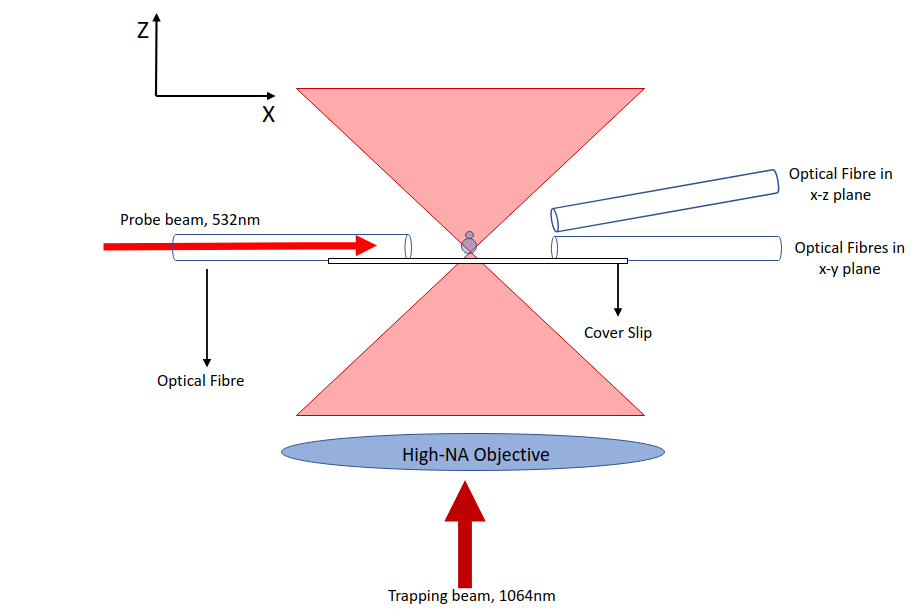
\includegraphics[width=\textwidth, height=0.25\textheight]{./Images/fig1a.png}
\end{subfigure}
\begin{subfigure}{0.45\textwidth}
	\subcaption{}
	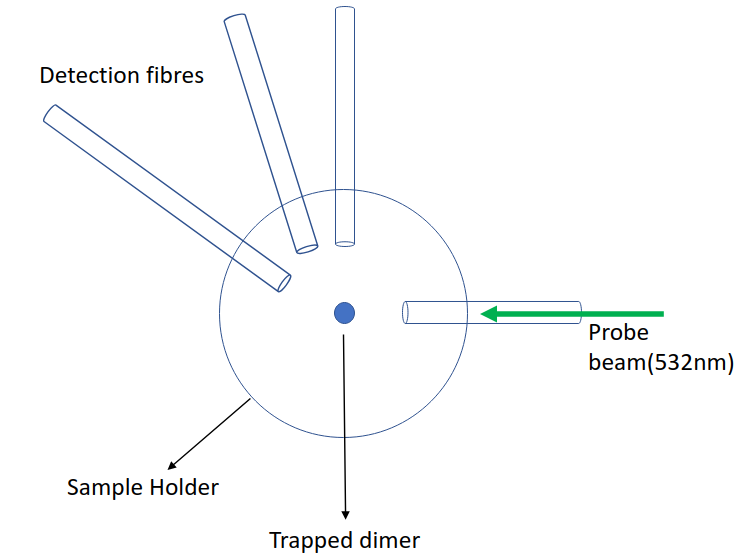
\includegraphics[width=\textwidth, height=0.25\textheight]{./Images/fig1b.png}
\end{subfigure}
\caption{\label{fig:setup}
  %
  Proposed experimental set up for scattering measurements from an object in an optical trap. The probe beam for scattering measurements is incident perpendicular to the trapping laser propagation direction. a) Side view. b) Top view. Note that three of the detector fibres are co-planar with the incident probe beam, while the fourth detector is placed out of the plane (see text).
%
}
\end{figure}

\printnomenclature[0.55in]

%%%%%%%%%%%%%%%%%%%%%%%%%%%%%%%%%%%%%%%%%%%%%%%%%%%%%%%%%%%%%%%%%%%%%%%%%%%%%%%%
%%%%%%%%%%%%%%%%%%%%%%%%%%%%%%%%%%%%%%%%%%%%%%%%%%%%%%%%%%%%%%%%%%%%%%%%%%%%%%%%
\section{Methodology}
\label{sec:Method}

\subsection{Brownian Simulation}
\label{sec:brownian}

We use the Brownian OT package developed by Fung~\textit{et~al} \cite{Vigilante2020Brownian_OT} to simulate the motion of an asymmetric dimer (Figure~\ref{fig:dimer}a) within an optical trap. Brownian OT combines MSTM \cite{Mishchenko1996MSTM} and ``Optical Tweezer Toolbox'' (\textit{ott}) \cite{Lenton2020} to simulate the motion of arbitrary
shaped sphere clusters. We simulate the motion of a dimer trapped in a highly focused Gaussian beam by calculating its diffusion tensor according to the analytical solutions provided by Nir and Acrivos \cite{nir_acrivos_1973}. For a dimer of arbitrary sized spheres the diffusion tensor - which describes the Cartesian forces and torques - is a 6 $\times$ 6 matrix:
\begin{align}
	\begin{pmatrix}
		F_x \\ F_y \\ F_z \\ T_x \\ T_y \\ T_z 
	\end{pmatrix}
	= \begin{pmatrix}
	a_1 &   0  &     0     &   0  & d_1 &     0 \\
	 0  &  a_1 &     0     & -d_1 &  0  &     0 \\
	 0  &   0  & a_1 + a_2 &   0  &  0  &     0 \\
	 0  & -d_1 &     0     &  b_1 &  0  &     0 \\
	d_1 &   0  &     0     &   0  & b_1 &     0 \\
	 0  &   0  &     0     &   0  &  0  & b_1 + b_2     
	\end{pmatrix}
	\begin{pmatrix}
		v_{k0} - V_k \\ v_{k0} - V_k \\ v_{k0} - V_k \\
		\omega_x - \Omega_x \\ \omega_y - \Omega_y \\ \omega_z - \Omega_z
	\end{pmatrix}
\end{align}

where each matrix component is scaled by a factor of $k_B T/\pi \eta$ When both sphere's are identically sized - as in Fung~\textit{et. al}'s work - $d_1$ goes to zero; however for our work with asymmetric spheres these components are significant enough to be considered. We simulated a silica dimer ($n = 1.45$) in a suspension of water ($n_{med} = 1.33$) over the course of $10 \ s$ with a simulation time step of $1 \times 10^{-5} \ s$.

\begin{figure}[h]
	\centering
	\begin{subfigure}{0.49\textwidth}
		\subcaption{}
		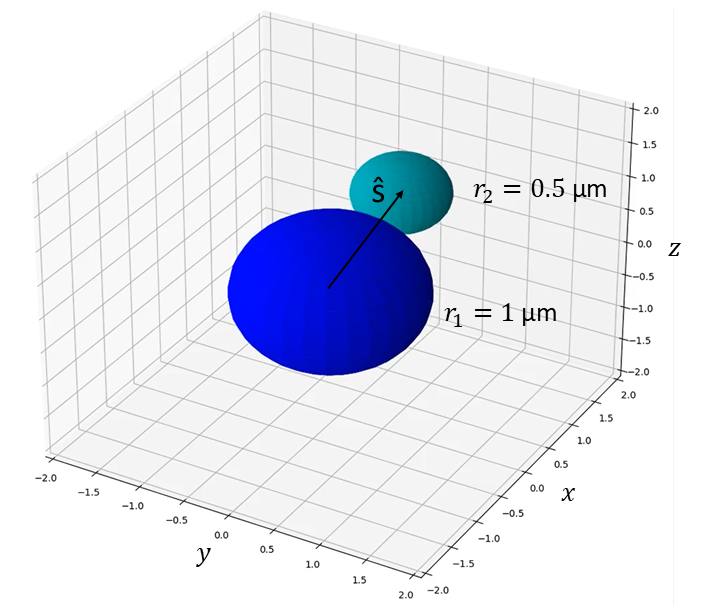
\includegraphics[width=\textwidth]{./Images/fig2a.png}
	\end{subfigure}
	\begin{subfigure}{0.49\textwidth}
		\subcaption{}
		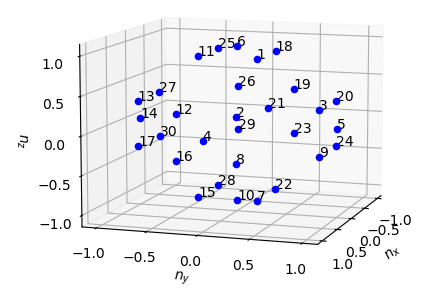
\includegraphics[width=\textwidth]{./Images/fig2b.png}
	\end{subfigure}
	\caption{(a)Example dimer in orientation $\bar{\bf s}$, (b) 30 Reference orientations represented by vectors pointing from [0,0,0] to each point}
	\label{fig:dimer}
\end{figure}

%%%%%%%%%%%%%%%%%%%%%%%%%%%%%%%%%%%%%%%%%%%%%%%%%%%%%%%%%%%%%%%%%%%%%%%%%%%%%%%%
\subsection{Orientation estimation from scattering measurements}
\label{sec:Bayes}

For our simulated dimer in the optical trap (Fig.~\ref{fig:dimer}a), we can define at any point in time a unit vector $\hat{s}$ pointing from the centre of the larger sphere to the centre of the smaller sphere. A plane wave 'probe' laser, perpendicular to the trapping laser, is incident on the dimer, generating a scattering pattern  dependent on the dimer's orientation $I(\hat{\bf s}, \theta)$ which is computed using MSTM. To represent the experimental set up consisting of a set of optical fibres recording scattered light, we choose four angles  ($\theta_1, \ \theta_2, \ \theta_3, \ \theta_4$) and record the calculated intensity at each angle $\theta_k$, $I(\hat{s}, \theta_k)$. 

Our goal is to determine the orientation of the trapped dimer based on the scattering data $I(\hat{n}, \ \theta_k)$. Rather than aim immediately for an exact estimate of the dimer's orientation, for the purposes of interpretation of the scattering and optimisation of the measurement setup it is more convenient to discretize the possible orientation space into a number of possible reference orientations, which we can then use as 'classification categories' in a neural network methodology to map scattering data to orientation (see below for further discussion).  Here we choose $\textit{n}_{ref} \ = \ 30$ reference orientations $\hat{\bf n}_{\alpha}$  evenly distributed on a unit sphere \cite{Rey2006} (Figure~\ref{fig:dimer}b) leading to a maximum nearest-neighbour spacing between two neighbouring reference orientations of 0.895 radians. Using MSTM we compute the raw intensities at each of the measurement angles that would be generated by a dimer in each reference orientation, $I(\hat{\bf n}_{\alpha}, \theta_k)$. While the number and position of detection fibres is technically arbitrary there are several constraining factors that limit our ability to infer useful information from the trapped object, see Section~\ref{sec:Discussion} for a detailed breakdown of our choice of detection angles. The raw intensities are normalized according to:
\begin{align}
\label{eq:scale}
  y_k(\hat{\bf n}_\alpha)
  = 
  \frac{I(\hat{\bf n}_\alpha, \theta_k) - \langle I(\hat{\bf n},\theta_k) \rangle } 
  {\langle I^2(\hat{\bf n},\theta_k) \rangle -\langle I(\hat{\bf n}, \theta_k)\rangle^2}
\end{align}
where the denominator is simply the standard deviation across the set of values $I(\hat{\bf n}, \theta_k)$. The reference orientations, raw intensities, and scaled signals are given in Tables~\ref{tab:A1} and \ref{tab:A2}. 

Note that the collected scattering signals are not necessarily simply related to their associated reference orientations: as is well known from such examples of the inverse scattering problem, the mapping between the structural space of variables such as orientation, and the space of scattering signals may be highly complex. Nevertheless, at least where the uncertainty in signal measurements is low (see below), we can predict the orientation from the scattering by utilising computational techniques such as neural networks. We thus utilised the Python machine learning program \textit{scikit-learn} to build a neural network for identifying the dimer's orientation from its light scattering signal. The network was trained by generating a database of random orientation vectors, calculating the corresponding light scattering signals, and then using the network to estimate the probability of a given signal coming from a dimer in a given reference orientation. The network's loss function was evaluated and used to improve the estimation, the network being trained until the improvement in the loss function was less than 0.0001. 
%
Importantly, the estimation provided by the neural network can be improved further by accounting for any prior information we know about the dimer,  utilising Bayesian inference to update the neural network's estimation: 

\begin{align}
  \label{eq:bayes}
  p(\hat{\bf n}_\alpha| y_k(\hat{\bf s}))
  &=
    \frac{p(y_k(\hat{\bf s})|\hat{\bf n}_\alpha)
    p(\hat{\bf n}_\alpha)}{p(y_k(\hat{\bf s}))}
\end{align}
where $p(\hat{\bf n}_\alpha)$ and $p(y_1, y_2, y_3)$ are the prior estimates of the distributions of particle orientations and instantaneous signals, respectively.
\textit{Without} any prior evidence we must assume that the orientation prior of the dimer
$p(\hat{\bf n}_{\alpha})$ is uniform. However, inference about the dimer's possible current orientation from knowledge of previous
measurements can be used to inform our estimate of $p(\hat{\bf n}_{\alpha})$ (see Section~\ref{sec:test}).  The latter prior $p(y)$ is the probability of measuring a signal ($y_1$, $y_2$, $y_3$).  This is given by taking the discrete integral over the collection of reference orientations:
\begin{align}
  p(y_1, y_2, y_3, y_4)
  =
  \sum_{\alpha=1}^{n_{\rm ref}}
  p(y_1, y_2, y_3, y_4|\hat{\bf n}_\alpha)
  p(\hat{\bf n}_\alpha)
\end{align}
From \eqref{eq:bayes} we obtain the key result, a mass probability distribution denoting the
probability that our dimer is in orientation $\hat{\bf n}_{\alpha}$ given a measured
signal ($y_1$, $y_2$, $y_3$), \textit{i.e.} an estimated mapping from scattering measurement to orientation estimate. 

%%%%%%%%%%%%%%%%%%%%%%%%%%%%%%%%%%%%%%%%%%%%%%%%%%%%%%%%%%%%%%%%%%%%%%%%%%%%%%%%
\subsection{Calculation of error}
\label{sec:divergence}
To evaluate the above estimation of dimer orientation from scattering signal, we use a Brownian simulation of a dimer in the optical trap (Section~\ref{sec:brownian}) to compare estimated most probable reference orientation, derived from the dimer's scattering through Eq.~\eqref{eq:bayes}, with the dimer's known \emph{actual} orientation $\hat{\bf s}$. MSTM provides calculated light scattering from the simulated dimer $I(\hat{\bf s}, \theta)$ and we use \eqref{eq:scale} to obtain normalized values at each measurement angle $\theta_k$,  $y_1(\hat{\bf s})$, $y_2(\hat{\bf s})$, $y_3(\hat{\bf s})$, from which we obtain $p(\hat{\bf n}_{\alpha}\parallel y_1, y_2, y_3)$. Because we know the actual orientation $\hat{s}$ we can measure the error in the model's estimate by comparing the reference orientation closest to $\hat{s}$, denoted as $\hat{\bf n}_{best}$, with the most probable predicted orientation from Eq.~\eqref{eq:bayes}. An ideal result would be one where the probability distribution is 0 for every $\hat{\bf n}$ apart from $\hat{\bf n}_{best}$:
\begin{align}
	\label{eq:best}
	p_{best} = 
	\begin{cases}
		1 & \text{when $\hat{\bf n}_\alpha$ = $\hat{\bf n}_{best}$}\\
		0 & \text{anywhere else}
	\end{cases}
\end{align}
In reality the distribution from Eq.~\eqref{eq:bayes} will assign some non-zero
probability to every reference orientation, leading to some level 'confidence' in orientation prediction, which can be quantified by calculating the Kullback-Leibler divergence $K_l$ between the two distributions:
\begin{align}
	K_{l, \#}(p_{best}\parallel p(\hat{\bf n}_\alpha| y_1, y_2, y_3))
	= p_{best}\ln \left[\frac{p_{best}}{p(\hat{\bf n}_{best}| y_1,y_2,y_3))}
	\right]
	\label{eq;kullback}
\end{align}
where a larger value of $K_l$ indicates that our model is less confident in its
prediction of the dimer's orientation. The divergence $K_l$ thus illustrates the 'spread'
in the estimated dimer orientation probability --- a distribution strongly peaked at 
some value would give us more confidence in that value than a near-uniform distribution 
where the scattering measurement could imply a wide range of possible orientations --- 
but it does not directly indicate our estimate's actual accuracy. 
%%%%%%%%%%%%%%%%%%%%%%%%%%%%%%%%%%%%%%%%%%%%%%%%%%%%%%%%%%%%%%%%%%%%%%%%%%%%%%%%
\section{Results and  Discussion}
\label{sec:Discussion}\subsection{Testing the Model}
\label{sec:test}
Using our simulation from Section~\ref{sec:brownian} we simulated the motion of a silica dimer ($n = 1.59$) trapped in water ($n = 1.33$) within a 5 mW optical trap. The trapping laser is 1064nm NIR focused through a 1.25 NA objective. The dimer is comprised of two tangent spheres with radii $1 \mu m$ and $0.5 \mu m$ respectively. We simulated the first 10 seconds of motion, calculating the orientation and position every 1 ms. 

We applied Eq.~\eqref{eq:bayes}, taking the reference orientation with the highest probability  as our estimate of the dimer's instantaneous orientation $\hat{\bf n}_{est}$. To visualise the model's performance  we plotted the radial distance between our estimation $\hat{\bf n}_{est}$ and the dimer's \emph{actual} instantaneous orientation $\hat{\bf s}$ versus time. For comparison, we also plotted the radian distance between the  dimer's instantaneous orientation and the closest reference orientation, denoted $\hat{\bf n}_{best}$. The dotted line indicates the maximum radian distance ($0.896$ radians) between two \textit{neighbouring} reference orientations: if we are under this line then we know our estimate is at least neighbouring the best result. Assuming a uniform prior of the reference orientations $p(\hat{\bf n}_\alpha)$  the neural network's predictions ($\hat{\bf n}_{est}$ from Eq.~\eqref{eq:bayes}) are at times reasonable, but there are significant large and random jumps away from the correct result (Fig.~\ref{fig:uniform}). 

\begin{figure}[h]
	\centering
	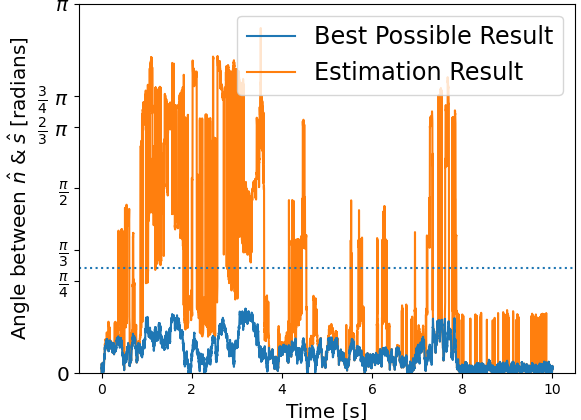
\includegraphics[width=0.5\textwidth]{./Images/fig3.png}
	\caption{Model's estimation of dimer orientation over the simulation time, assuming uniform prior $p(\hat{\bf n}_\alpha)$. Blue line denotes the best result we can achieve (the reference orientation $\hat{\bf n}_{best}$ that is closest to the actual orientation), orange line denotes the result provided by eq~\ref{eq:bayes}: where the orange line is not visible, the model's prediction agrees with $\hat{\bf n}_{best}$. Horizontal dotted line denotes maximum spacing between two neighbouring $\hat{\bf n}_\alpha$.}
	\label{fig:uniform}
\end{figure} 

One reason we observe such large jumps in  orientation estimated from scattering signals is that there is no simple correlation between the 'distance in scattering space' between scattering signals from two different orientations, and their separation in orientation space : even a large change in orientation can involve a small change in scattering. Combining this fact with use of a uniform prior, indicating essentially no knowledge of how orientation should behave, there is no constraint on how much estimated orientation can change from time-step to time-step. To improve the estimation we can therefore use knowledge of the physical limitations of the object in the trap and its dynamics, imposing a more physically grounded prior,  accounting in this case for the fact that the motion of the dimer is limited due to the trap stiffness. Here the prior of the reference orientations $p(\hat{\bf n}_\alpha)$ was redefined at each time step according to the physical distance between the previous estimate $\hat{\bf n}_{est}(t-\Delta t)$ and each reference orientation $\hat{\bf n}_\alpha$, \textit{i.e.} taking into account the different likelihoods of the estimated orientation jumping between nearby or distant reference orientations:

\begin{align}
  p(\hat{\bf n}_\alpha)
  &=\frac{e^{\beta (\hat{\bf n}_\alpha 
  	\cdot \hat{\bf n}_{est}(t-\Delta t))}}
  {\sum_{\alpha=1}^{n_{\rm ref}}
	e^{\beta (\hat{\bf n}_\alpha 
	\cdot \hat{\bf n}_{est}(t-\Delta t)}}
	\label{eq:boltz}
\end{align}
Here $\beta$ is a weighting factor describing the dimer's freedom of motion within the trap. As shown in Figure~\ref{fig:biased} implementation of Eq~\eqref{eq:boltz} helps significantly reduce the large random excursions of estimated orientation away from the 'best' result. 

\begin{figure}[h]
\centering
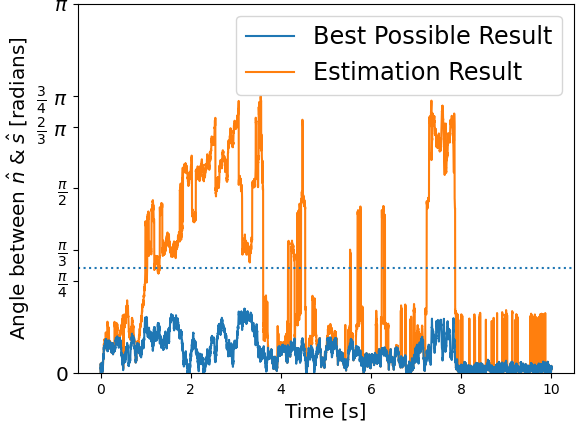
\includegraphics[width=0.5\textwidth]{./Images/fig4.png}
\caption{\label{fig:biased}
%
Estimation of dimer orientation with $p(\hat{\bf n}_\alpha)$ defined
by Eq~\eqref{eq:boltz}.  Blue line denotes the best result we can
achieve, orange line denotes the result provided by eq~\ref{eq:bayes}.
Dotted line denotes spacing between two neighbouring reference
orientations $\hat{\bf n}_\alpha$ (see Section~\ref{sec:Bayes}).
  %
}
\end{figure} 
 


The simulation data from Section~\ref{sec:brownian} was used to evaluate our model's performance --- covered in Section~\ref{sec:divergence}. By summing the divergence of each measurement across the entire simulation we get an evaluation of how well the model performed in estimating the dimer's orientation. To compare the effects of changing certain parameters on the performance of our model we compare our result of $K_{l,total}$ to a worst case scenario and evaluate how much it improves upon this, denoted as $F(K_l)$:
\begin{align}
  K_{l, \ total} &= \sum\limits_{\# =1}^{timesteps} K_{l,\#}
  \\
  K_{l, \ worst} &= \sum\limits_{\#=1}^{timesteps} \ln \left[\frac{1}{1/n_{ref}} \right]
  \\
F(K_l) &= \frac{K_{l,\ worst}}{K_{l, \ total}}
\end{align}

The worst case scenario is akin to randomly choosing a reference
orientation at each time step. The greater the value of $F(K_l)$, the
better our model's confidence is in characterising the dimer's
motion. Because our model is dependent on several parameters we need
to a sophisticated method for understanding how these parameters
correlate with $F(K_l)$.


%%%%%%%%%%%%%%%%%%%%%%%%%%%%%%%%%%%%%%%%%%%%%%%%%%%%%%%%%%%%%%%%%%%%%%%%%%%%%%%%
%%%%%%%%%%%%%%%%%%%%%%%%%%%%%%%%%%%%%%%%%%%%%%%%%%%%%%%%%%%%%%%%%%%%%%%%%%%%%%%%
\subsection{Asymmetric dimer dynamics}
\label{sec:motion}

The Brownian OT software was used to simulate the motion of a trapped
dimer ($a_1=1\,\mu{\rm m}$, $a_2=0.5\,\mu{\rm m}$) over the first
$10$ seconds of entering the optical trap.  The initial orientation
was assumed as strictly vertical (in line with the beam propagation
direction). The dimer's position and orientation was recorded every
$1\,{\rm ms}$ for using as a test dataset for our model.


\begin{figure}[h]
	\centering
	\begin{subfigure}{0.45\textwidth}
		\subcaption{}
		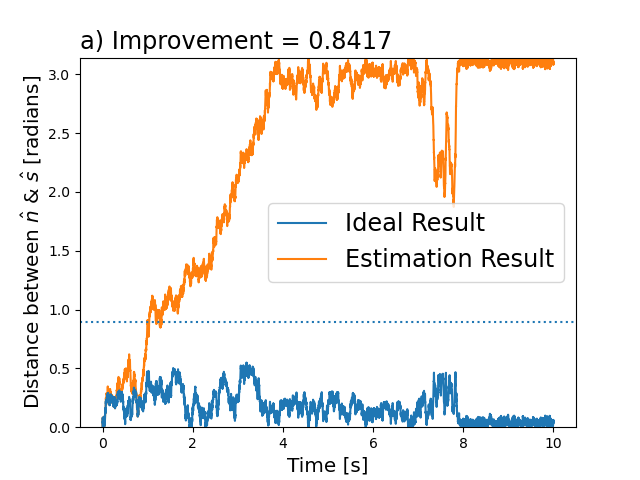
\includegraphics[width =\textwidth]{./Images/fig5a.png}
	\end{subfigure}
	\begin{subfigure}{0.45\textwidth}
		\subcaption{}
		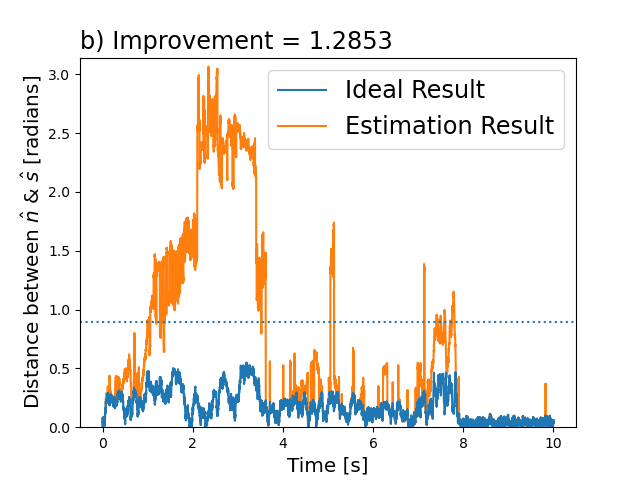
\includegraphics[width=\textwidth]{./Images/fig5b.png}
	\end{subfigure}
	\caption{Simulation results of: (a) the dimer's orientation vector with time, (b) the dimer's [x,y,z] position with time.}
	\label{fig:motion}
\end{figure}

As can be seen from Figure~\ref{fig:motion}, the dimer undergoes a full $180^{\circ}$ rotation upon entering the trap.  Typically horizontal alignment of a dimer is unstable and will result in the particle rotating to align along its vertical axis.  It is interesting to note that the dimer is furthest from the trap centre as it reaches a horizontal orientation before drawing closer again as it inverts completely. Further simulations of dimers with different size ratio $a_1 \geq 2a_2$ showed a similar behaviour of initially moving away from the trap focus and rotating while remaining trapped before re-aligning, while dimers with size ratis $a_1 < 2a_2$ immediately aligned into a fixed vertical position.
%
In the simulations of Vigilante~\emph{et~al}.\ \cite{Vigilante2020Brownian_OT}, trapped symmetrical dimers were investigated; their findings showed that the optical torque on the dimer goes to zero while aligned vertically and is at its maximum in a horizontal alignment. Therefore, the inversion of an asymmetric dimer suggests that if the size difference is significant the optical torque is minimal for a dimer in both horizontal and vertical orientations.  
%%%%%%%%%%%%%%%%%%%%%%%%%%%%%%%%%%%%%%%%%%%%%%%%%%%%%%%%%%%%%%%%%%%%%%%%%%%%%%%%
\subsection{Impact of measurement noise on model predictions}
\label{sec:epsilon}

So far a key assumption of the neural network implementation is that the detected scattering signal  has no uncertainty associated with it. In reality of course detected scattering signals  will have some non-zero level of measurement  noise. To explore the impact of measurement uncertainty on orientation estimation model performance we introduce a Gaussian noise to the measured signal:
\begin{align}
	I(\hat{\bf s}) = I(\hat{\bf s}) \pm \epsilon I(\hat{\bf s})
\end{align}
where $\epsilon$ is the percentage error associated with the scattering signal.  Figure~\ref{fig:epsilon} shows the performance of the model at a range of $\epsilon$ using in-plane detector angles $15^{\circ}$, $55^{\circ}$, $90^{\circ}$ and out-of-plane detector at $75^{\circ}$, with $\beta$ set to $1$:

\begin{figure}[h]
	\centering
	\begin{subfigure}{0.32\textwidth}
		\subcaption{}
		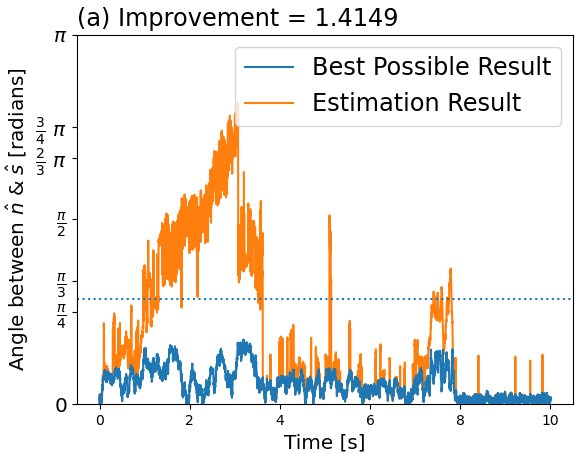
\includegraphics[width=\textwidth]{./Images/fig6a.png}
	\end{subfigure}
	\begin{subfigure}{0.32\textwidth}
		\subcaption{}
		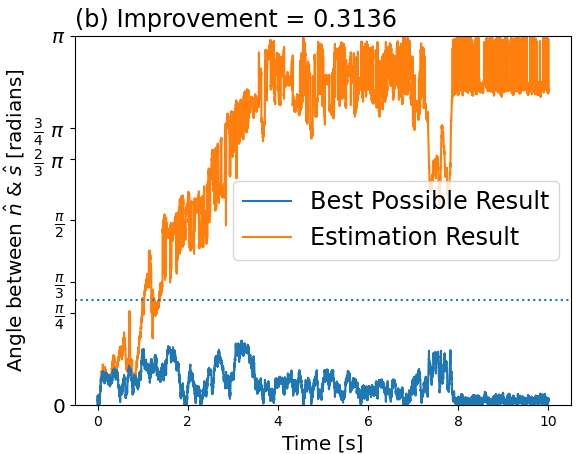
\includegraphics[width=\textwidth]{./Images/fig6b.png}
	\end{subfigure}
	\begin{subfigure}{0.32\textwidth}
		\subcaption{}
		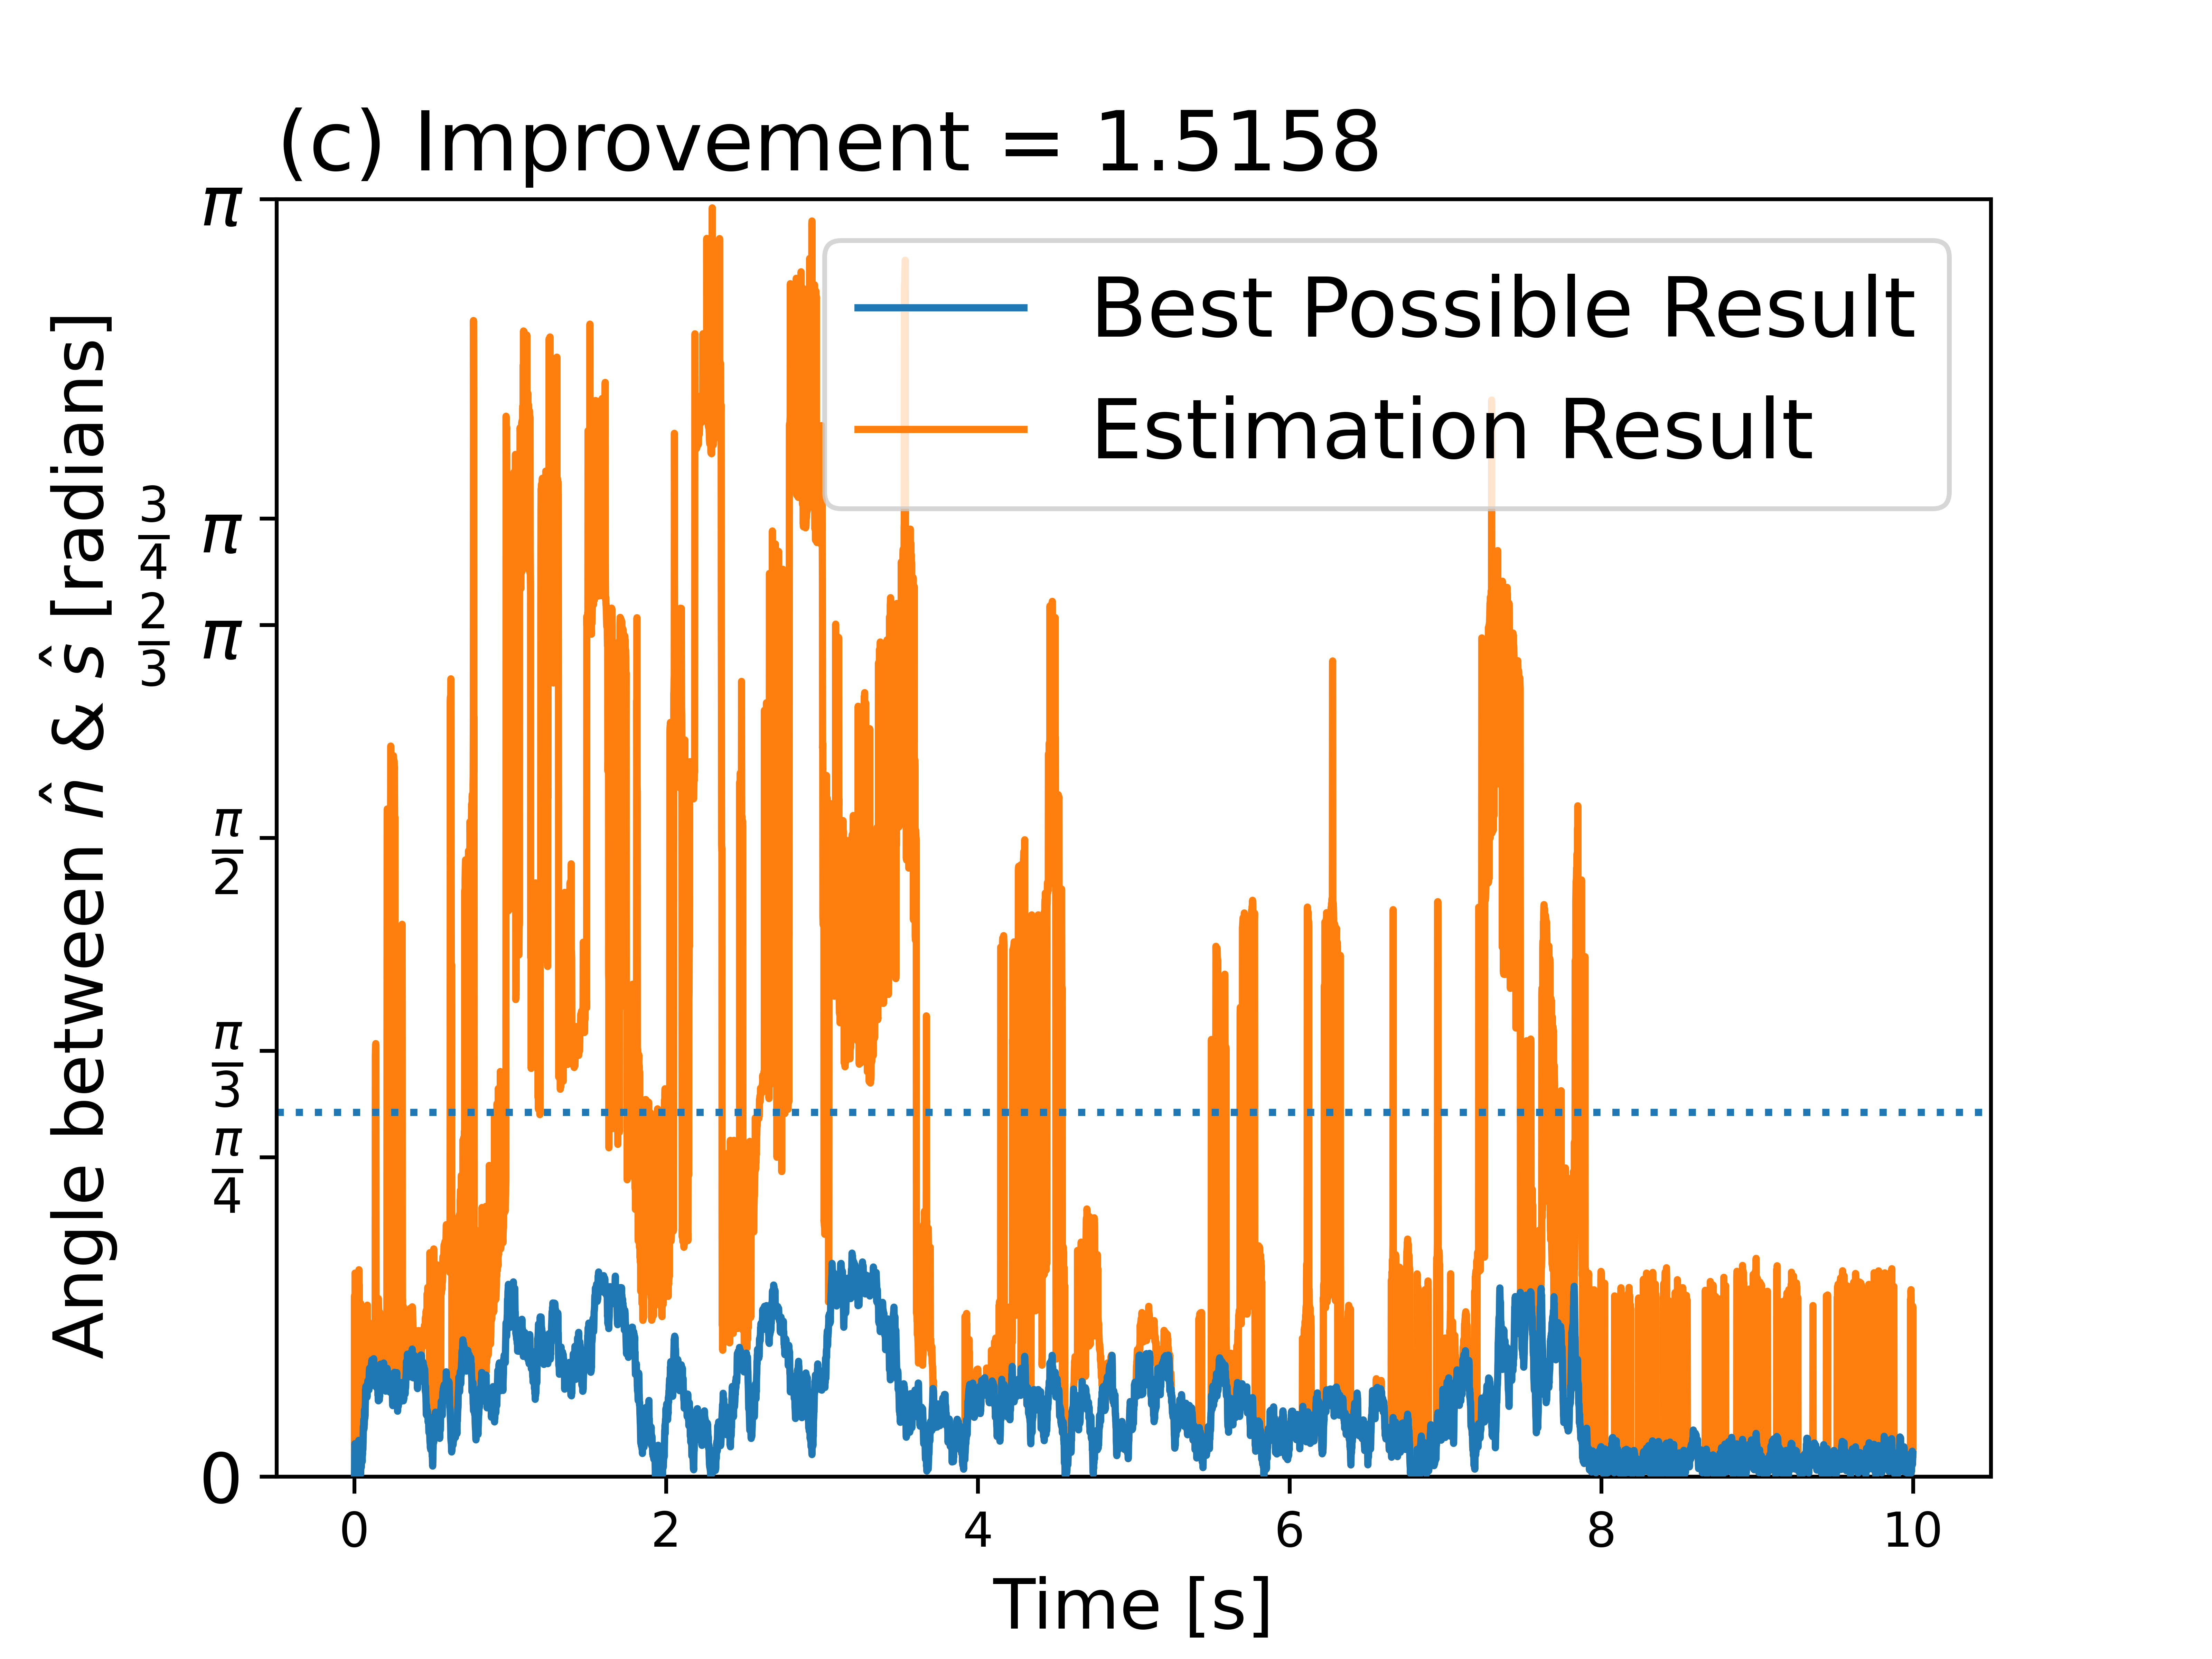
\includegraphics[width=\textwidth]{./Images/fig6c.png}
	\end{subfigure}
	\caption{Model prediction for signal error of (a) $1\%$ ~  $[F(K_l)=1.174]$, (b) $15\%$ ~ [$[F(K_l)=0.606]$, and (c) $25\%$ ~  $[F(K_l)=0.457]$.}
	\label{fig:epsilon}
\end{figure}

As can be seen from Figure~\ref{fig:epsilon}, the inclusion of signal noise quickly leads to a decrease in the model's performance. This is due to an inherent feature of the inverse scattering problem: two distinct regions in orientation space can become heavily intertwined and thus no longer well separated when mapped to intensity space (even though the mapping remains  continuous): so even small uncertainties in the scattering data can lead to large 'mistakes' in the choice of orientation by the neural network. (Indeed if this was not the case the inverse scattering problem would be quite simple.) Fortunately, we can alleviate the impact of signal noise by increasing the weighting factor $\beta$ reflecting the degree of freedom the dimer has within the trap, once again because we know that for a given trap strength, large rapid changes in the dimer orientation are physically limited. We show model results for the same signal noise as Fig.~\ref{fig:epsilon} but with increasing $\beta$ in Figure~\ref{fig:beta}.

\begin{figure}[h]
	\centering
	\begin{subfigure}{0.32\textwidth}
		\subcaption{}
		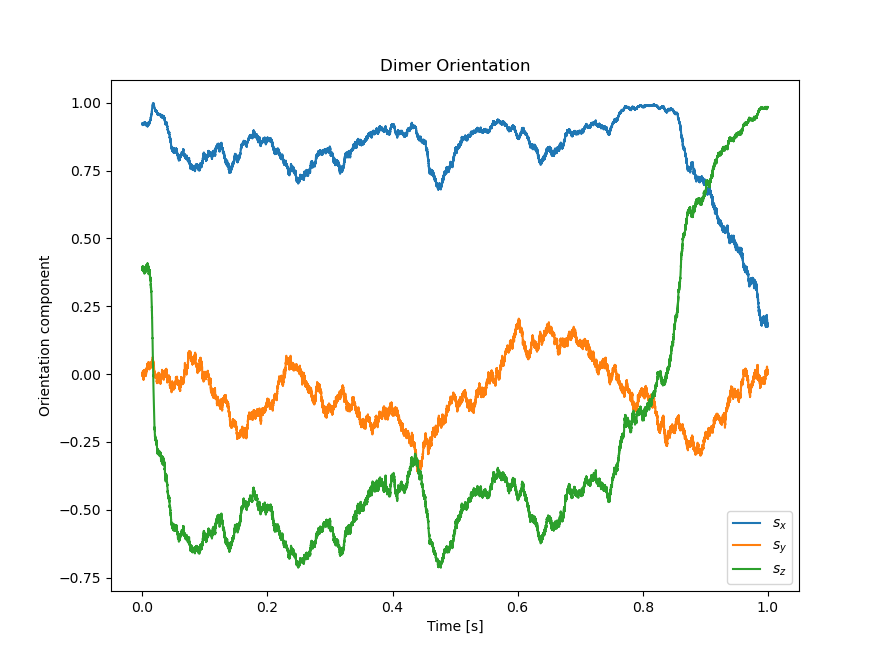
\includegraphics[width=\textwidth]{./Images/fig7a.png}
	\end{subfigure}
	\begin{subfigure}{0.32\textwidth}
		\subcaption{}
		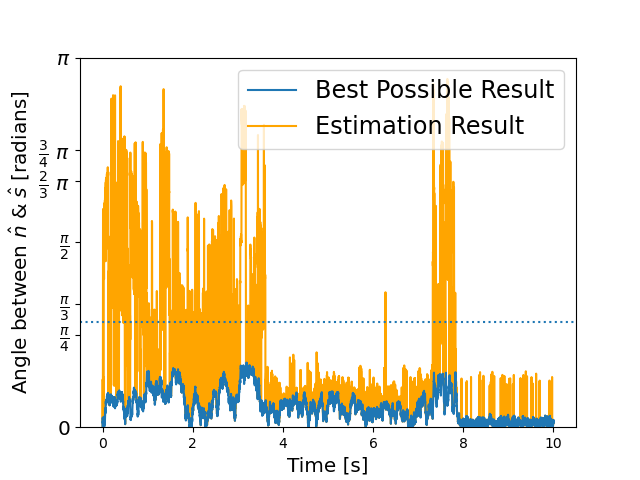
\includegraphics[width=\textwidth]{./Images/fig7b.png}
	\end{subfigure}
	\begin{subfigure}{0.32\textwidth}
		\subcaption{}
		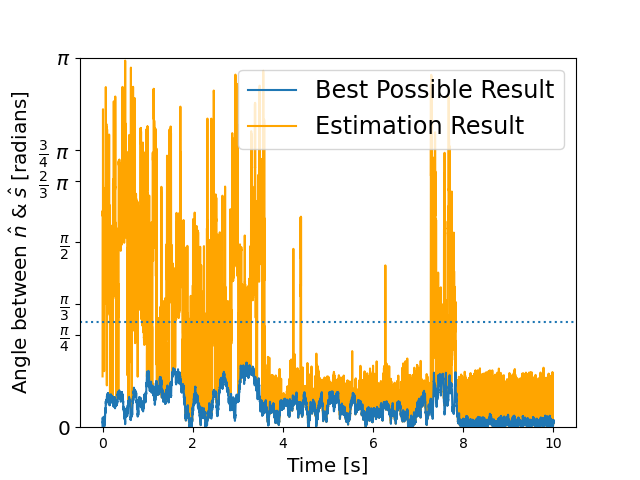
\includegraphics[width=\textwidth]{./Images/fig7c.png}
	\end{subfigure}
	\caption{Model prediction for signal noise $\epsilon$ of $1\%$, $15\%$, and $25\%$ with (a) $\beta=4$ ~ $[F(K_l)=1.914]$, (b) $\beta=15$ ~  $[F(K_l)=0.734]$, and (c) $\beta=22$ ~ $[F(K_l)=0.621]$.} 
	\label{fig:beta}
\end{figure}

Increasing $\beta$ helps significantly reduce the random fluctuations in the model. Of course, at too high a $\beta$ the orientation estimation will be 'over-corrected' \textit{i.e.} real changes in orientation indicated by real changes in scattering, as opposed to noise, will be suppressed. The exact value of $\beta$ that will best optimise model performance varies based on the expected signal error and the actual trap strength and trapped object dynamics, therefore  it can be used as a variable for 'intelligently' fine tuning results from the neural network and Bayesian inference, using the details of the trap setup and measurement system as essentially 'prior knowledge'. 


%%%%%%%%%%%%%%%%%%%%%%%%%%%%%%%%%%%%%%%%%%%%%%%%%%%%%%%%%%%%%%%%%%%%%%%%%%%%%%%%
%%%%%%%%%%%%%%%%%%%%%%%%%%%%%%%%%%%%%%%%%%%%%%%%%%%%%%%%%%%%%%%%%%%%%%%%%%%%%%%%
\section{Conclusion}
\label{sec:Conclusion}

We have developed a method for measuring the dynamics of an optically-trapped 'complex object' based purely on limited measurements of the object's light scattering at a small number of detection angles. We demonstrate the method using the orientation of an asymmetric dimer as the dynamical variable and object of interest, but in principle the model can be applied to any characteristic that impacts the light scattering pattern produced by a trapped entity. The MSTM package is a flexible tool for calculating the light scattering of complex objects using a representation of the object as a set of micro-particles, enabling training of a neural network to enable categorisation of the mapping between scattering and trapped object characteristics. By taking account of knowledge about the physically realistic behaviour of the trapped object and the characteristics of the trap (which impact the dynamics of the object), the Bayesian inference method can be refined to provide a reliable estimation of object characteristics of interest, even in the presence of measurement noise. Fundamentally the inverse scattering problem is difficult to solve since the mapping between object characteristics and scattering can be highly complex: but Bayesian inference based on neural network estimation of the mapping provides a powerful method for practical applications, extending the use of optical trapping beyond measuring microscopic force response toward detailed structural and dynamic information about complex trapped entities.\\

Here we simplify the problem somewhat by employing a relatively small finite number of 'reference orientations' to map between scattering and dimer orientation: the precision of estimation could be improved by utilising a greater number of reference orientations, although there remains a balance between the realisable precision of orientation estimate and the noise level of the scattering measurement. Another avenue to further explore would be using the method to optimise the choice of detection angles, essentially to find the region in the mapping between measured scattering and orientation that offers the best degree of confidence through optimal separation of scattering signals for distinct orientations. For \textit{sequences} of data such as dynamic measurements, a further potential enhancement would be to consider more complex correlations based on prior expectations of the dynamics. Here already we improve the method using a non-uniform prior based on only the immediately previous measurement in time (see Section \ref{sec:Bayes}): considering more detailed correlations such as multiple previous timesteps is likely to further enhance the reliability of the estimation.


%%%%%%%%%%%%%%%%%%%%%%%%%%%%%%%%%%%%%%%%%%%%%%%%%%%%%%%%%%%%%%%%%%%%%%%%%%%%%%%%
%%%%%%%%%%%%%%%%%%%%%%%%%%%%%%%%%%%%%%%%%%%%%%%%%%%%%%%%%%%%%%%%%%%%%%%%%%%%%%%%
\noindent \textbf{Acknowledgement.} The authors thank the support for this research from the funding provided by the Leverhulme Trust. \\
  
\noindent \textbf{Disclosures.} The authors declare no conflict of interest. \\


%%%%%%%%%%%%%%%%%%%%%%%%%%%%%%%%%%%%%%%%%%%%%%%%%%%%%%%%%%%%%%%%%%%%%%%%%%%%%%%%
%%%%%%%%%%%%%%%%%%%%%%%%%%%%%%%%%%%%%%%%%%%%%%%%%%%%%%%%%%%%%%%%%%%%%%%%%%%%%%%%
\bibliography{bib} 
\bibliographystyle{ieeetr}

\newpage
\appendix
\onecolumn
%%%%%%%%%%%%%%%%%%%%%%%%%%%%%%%%%%%%%%%%%%%%%%%%%%%%%%%%%%%%%%%%%%%%%%%%%%%%%%%%
%%%%%%%%%%%%%%%%%%%%%%%%%%%%%%%%%%%%%%%%%%%%%%%%%%%%%%%%%%%%%%%%%%%%%%%%%%%%%%%%
\section*{Appendix}
\setcounter{table}{0}
\renewcommand{\thetable}{A\arabic{table}}
\begin{table}[h]
\begin{center}
\caption{\label{tab:A1}
%
Reference Orientations vector components$^*$}
\begin{tabular}{|c|c|c|c|}
\hline\hline
$\alpha$ & $\hat{\bf n}_{\alpha,\ x}$ &  $\hat{\bf n}_{\alpha,\ y}$ &  $\hat{\bf n}_{\alpha,\ z}$ \\
\hline
$1$  & $ 0.29588$ &  $ 0.29588$ & $ 0.90825$ \\
$2$  & $ 0.90825$ &  $ 0.29588$ & $ 0.29588$ \\
$3$  & $ 0.29588$ &  $ 0.90825$ & $ 0.29588$ \\
$4$  & $ 1.00000$ &  $ 0.00000$ & $ 0.00000$ \\
$5$  & $ 0.00000$ &  $ 1.00000$ & $ 0.00000$ \\
$6$  & $ 0.00000$ &  $ 0.00000$ & $ 1.00000$ \\
$7$  & $ 0.29588$ &  $ 0.29588$ & $-0.90825$ \\
$8$  & $ 0.90825$ &  $ 0.29588$ & $-0.29588$ \\
$9$  & $ 0.29588$ &  $ 0.90825$ & $-0.29588$ \\
$10$ & $ 0.00000$ &  $ 0.00000$ & $-1.00000$ \\
$11$ & $ 0.29588$ &  $-0.29588$ & $ 0.90825$ \\
$12$ & $ 0.90825$ &  $-0.29588$ & $ 0.29588$ \\
$13$ & $ 0.29588$ &  $-0.90825$ & $ 0.29588$ \\
$14$ & $ 0.00000$ &  $ -1.0000$ & $ 0.00000$ \\
$15$ & $ 0.29588$ &  $-0.29588$ & $-0.90825$ \\
$16$ & $ 0.90825$ &  $-0.29588$ & $-0.29588$ \\
$17$ & $ 0.29588$ &  $-0.90825$ & $-0.29588$ \\
$18$ & $-0.29588$ &  $ 0.29588$ & $ 0.90825$ \\
$19$ & $-0.90825$ &  $ 0.29588$ & $ 0.29588$ \\
$20$ & $-0.29588$ &  $ 0.90825$ & $ 0.29588$ \\
$21$ & $-1.00000$ &  $ 0.00000$ & $ 0.00000$ \\
$22$ & $-0.29588$ &  $ 0.29588$ & $-0.90825$ \\
$23$ & $-0.90825$ &  $ 0.29588$ & $-0.29588$ \\
$24$ & $-0.29588$ &  $ 0.90825$ & $-0.29588$ \\
$25$ & $-0.29588$ &  $-0.29588$ & $ 0.90825$ \\
$26$ & $-0.90825$ &  $-0.29588$ & $ 0.29588$ \\
$27$ & $-0.29588$ &  $-0.90825$ & $ 0.29588$ \\
$28$ & $-0.29588$ &  $-0.29588$ & $-0.90825$ \\
$28$ & $-0.90825$ &  $-0.29588$ & $-0.29588$ \\
$30$ & $-0.29588$ &  $-0.90825$ & $-0.29588$ \\
\hline\hline
\multicolumn{4}{l}{\small *Orientation vector points from centre of sphere 1 to centre of sphere 2.} \\
		\end{tabular}
	\end{center}
\label{sec:App1}
\end{table}


\newpage
%%%%%%%%%%%%%%%%%%%%%%%%%%%%%%%%%%%%%%%%%%%%%%%%%%%%%%%%%%%%%%%%%%%%%%%%%%%%%%%%
\begin{table}[h]
  \begin{center}
    \caption{\label{tab:A2}
      % 
      Raw intensities $I_k^*$ and scaled intensities $y_k$}
    \begin{tabular}{|c|c|c|c|c|c|c|}
      \hline\hline
      $\alpha$  & $I(\hat{\bf n}_\alpha\ ,\ 15^{\circ})$ &  $I(\hat{\bf n}_\alpha \ , \ 55^{\circ})$ &  $I(\hat{\bf n}_\alpha \ ,\ 90^{\circ})$ & $y(\hat{\bf n}_\alpha \ , \ 15^{\circ})$ & $y(\hat{\bf n}_\alpha \ , \ 55^{\circ})$ & $y(\hat{\bf n}_\alpha \ , \ 90^{\circ})$ \\
\hline
$1$  & $5.6777$ & $0.0180$ & $0.0122$ & $-0.3137$ & $-0.6242$ & $-0.4838$ \\
$2$  & $5.2364$ & $0.0088$ & $0.0102$ & $-0.5663$ & $-0.8951$ & $-0.7826$ \\
$3$  & $9.0297$ & $0.0141$ & $0.0234$ & $ 1.6044$ & $-0.7378$ & $ 1.1622$ \\
$4$  & $4.5187$ & $0.0459$ & $0.0221$ & $-0.9770$ & $ 0.2062$ & $ 0.9695$ \\
$5$  & $8.5891$ & $0.0392$ & $0.0244$ & $ 1.3523$ & $ 0.0060$ & $ 1.3031$ \\
$6$  & $7.1799$ & $0.0377$ & $0.0142$ & $ 0.5458$ & $-0.0383$ & $-0.1886$ \\
$7$  & $5.0015$ & $0.0071$ & $0.0095$ & $-0.7007$ & $-0.9468$ & $-0.8792$ \\
$8$  & $4.8573$ & $0.0578$ & $0.0095$ & $-0.7832$ & $ 0.5604$ & $-0.8794$ \\
$9$  & $9.0184$ & $0.0618$ & $0.0273$ & $ 1.5979$ & $ 0.6774$ & $ 1.7262$ \\
$10$ & $4.6351$ & $0.1536$ & $0.0221$ & $-0.9103$ & $ 3.4040$ & $ 0.9641$ \\
$11$ & $5.6777$ & $0.0180$ & $0.0122$ & $-0.3137$ & $-0.6242$ & $-0.4838$ \\
$12$ & $5.2364$ & $0.0088$ & $0.0102$ & $-0.5663$ & $-0.8951$ & $-0.7826$ \\
$13$ & $9.0297$ & $0.0141$ & $0.0234$ & $ 1.6044$ & $-0.7378$ & $ 1.1622$ \\
$14$ & $8.5891$ & $0.0392$ & $0.0244$ & $ 1.3523$ & $ 0.0060$ & $ 1.3031$ \\
$15$ & $5.0015$ & $0.0071$ & $0.0095$ & $-0.7007$ & $-0.9468$ & $-0.8792$ \\
$16$ & $4.8573$ & $0.0578$ & $0.0095$ & $-0.7832$ & $ 0.5604$ & $-0.8794$ \\
$17$ & $9.0184$ & $0.0618$ & $0.0273$ & $ 1.5979$ & $ 0.6774$ & $ 1.7262$ \\
$18$ & $7.1549$ & $0.0408$ & $0.0076$ & $ 0.5315$ & $ 0.0532$ & $-1.1580$ \\
$19$ & $4.0546$ & $0.0085$ & $0.0076$ & $-1.2425$ & $-0.9035$ & $-1.1576$ \\
$20$ & $5.9164$ & $0.0122$ & $0.0188$ & $-0.1771$ & $-0.7945$ & $ 0.4765$ \\
$21$ & $4.2902$ & $0.0103$ & $0.0142$ & $-1.1077$ & $-0.8510$ & $-0.1890$ \\
$22$ & $7.9307$ & $0.1005$ & $0.0102$ & $ 0.9754$ & $ 1.8281$ & $-0.7835$ \\
$23$ & $4.0693$ & $0.0414$ & $0.0122$ & $-1.2342$ & $ 0.0718$ & $-0.4840$ \\
$24$ & $6.5422$ & $0.0506$ & $0.0234$ & $ 0.1809$ & $ 0.3446$ & $ 1.1622$ \\
$25$ & $7.1549$ & $0.0408$ & $0.0076$ & $ 0.5315$ & $ 0.0532$ & $-1.1580$ \\
$26$ & $4.0546$ & $0.0085$ & $0.0076$ & $-1.2425$ & $-0.9035$ & $-1.1576$ \\
$27$ & $5.9164$ & $0.0122$ & $0.0188$ & $-0.1771$ & $-0.7945$ & $ 0.4765$ \\
$28$ & $7.9307$ & $0.1005$ & $0.0102$ & $ 0.9754$ & $ 0.1005$ & $ 0.0102$ \\
$29$ & $4.0693$ & $0.0414$ & $0.0122$ & $-1.2342$ & $ 0.0718$ & $-0.4840$ \\
$30$ & $6.5422$ & $0.0506$ & $0.0234$ & $ 0.1809$ & $ 0.3446$ & $ 1.1622$ \\
\hline\hline
\multicolumn{7}{l}{\small *$I_k$ values are calculated using MSTM package.}
\end{tabular}
\end{center}
\label{sec:App2}
\end{table}


%%%%%%%%%%%%%%%%%%%%%%%%%%%%%%%%%%%%%%%%%%%%%%%%%%%%%%%%%%%%%%%%%%%%%%%%%%%%%%%%
%%%%%%%%%%%%%%%%%%%%%%%%%%%%%%%%%%%%%%%%%%%%%%%%%%%%%%%%%%%%%%%%%%%%%%%%%%%%%%%%
%%%%%%%%%%%%%%%%%%%%%%%%%%%%%%%%%%%%%%%%%%%%%%%%%%%%%%%%%%%%%%%%%%%%%%%%%%%%%%%%
\end{document}
\endinput
